\documentclass[10pt,journal]{IEEEtran}
\usepackage{microtype}
\usepackage{amsmath,amssymb,mathtools}
\usepackage{booktabs,multirow,array}
\usepackage{graphicx}
\usepackage{cite}
\usepackage{xcolor}
\usepackage{url}
\emergencystretch=1em
% Standard IEEEtran font sizes and baseline are retained throughout.
\setlength{\textfloatsep}{8pt plus 2pt minus 2pt}
\setlength{\floatsep}{7pt plus 2pt minus 2pt}
\setlength{\intextsep}{8pt plus 2pt minus 2pt}
\renewcommand{\arraystretch}{1.08}
\newcommand{\RiskSafe}{joint-risk verifier}
\newcommand{\TailRisk}{tail-only verifier}
\newcommand{\PaymentSafe}{value-certified verifier}
\newcommand{\dt}{\Delta t}

\title{Workload-State Verification and Security-Aware\\
Settlement for Spatially Coupled Data Centers}
\author{Anonymous Authors}

\begin{document}
\maketitle

\begin{abstract}
Artificial-intelligence data centers can provide demand response, but a meter
reduction alone establishes neither workload commitment nor positive grid
value. This paper develops a declaration-indexed verification and settlement
framework that connects risk budgets, executable jobs, and network value.
An exact convex accuracy constraint and an active tail-risk budget define a
validation-fitted contract. A residual certificate bounds risk and accuracy
changes during execution; an integer formulation jointly enforces continuous
job runtimes, site capacity, scenario risk, and exact lattice-based error.
Signed nodal valuation includes spatial rebound, while a closed-meter
intersection limits payable credit. In a retrospective 54-day comparison,
the active-tail formulation reduces mean false credit from 0.565 to
0.540 MWh/day relative to its matched total-only control; the tail difference
remains statistically unresolved. Twenty-four coupled runtime cases attain
zero optimization gap, and phase-I solves identify the accuracy attainable
under binding capacity. A common-domain AC audit retains all 10,332 cells,
including 690 numerical unknowns, rather than changing the comparison domain.
These results establish explicit contract-admission conditions and reproducible
security accounting. Public traces support modeled and observational audits;
prospective utility-event evidence is still required for deployment validation.
\end{abstract}

\noindent\textbf{Index Terms---}AI data centers, counterfactual verification,
demand response, security-constrained dispatch, nodal settlement.

\section{Introduction}

Data centers can shift computing work across time and regions, creating a
software-defined source of demand response (DR). Yet a decrease at one meter
may coincide with deferred consumption or a load increase at another node.
Positive-only local accounting can therefore reward a redistribution with
little or negative grid value. Public traces expose multi-week bursty arrivals
and scheduler jobs, but measure GPU energy at a different boundary from
whole-facility demand \cite{wang2024burstgpt,samsi2021supercloud}. A useful
verification protocol must connect these boundaries without equating them.

Historical baselines remain common in market practice
\cite{caiso2017baseline}; strategic consumption can manipulate their rewards
\cite{wang2022baseline}. A meter estimator alone cannot establish that
submitted jobs could generate its predicted profile. Workload scheduling and
computation--power models already establish temporal deferral, geographical
balancing, and grid coordination \cite{cao2022flexibility,li2024computation}.
Han et al. incorporate conditional value at risk (CVaR) into cross-regional
dispatchable-capacity assessment \cite{han2026dispatchable}. Here the risk
object is instead verification loss: total and daily-tail false credit,
subject to an accuracy neighborhood on the same declaration-based profiles.

Network-aware remuneration is also established. Chen et al. combine
IDC-aware optimal power flow, locational prices, net-benefit activation, and
benefit redistribution \cite{chen2021incentive}. Virtual links remunerate
space--time transfers using nodal price differences
\cite{zhang2020virtuallinks,zhang2022remunerating}; receding-horizon control
retains multi-site state and future arrivals \cite{zhang2023receding}.
Consequently, spatial scheduling, CVaR, and network compensation alone are not
our novelty claim. We test a declaration-indexed interface connecting these
layers, including where a guarantee does and does not survive conversion
between aggregate verification, discrete execution, and settlement.

The study makes three contributions:
\begin{enumerate}
\item A typed workload-to-network interface preserves declared job identity,
energy, release/deadline feasibility, and regional mapping. Its explicit
information gate separates deployable commitments from complete-ledger
ex-post comparators; a closed meter is required for payment.
\item A joint total-and-tail risk contract is combined with a contiguous-runtime
scheduler and a residual-based composition certificate. This distinguishes
optimality for a declared scheduling objective from preservation of the
statistical target, risk budgets, or accuracy guarantee. Matched-gate and
capacity-stress tests examine the assumptions needed for deployment.
\item Signed nodal and N--1 value are evaluated on the resulting workload
profiles, with a finite-scenario value cap and separate meter-backed capacity
payment. Common-denominator security checks preserve numerical failures
instead of screening them out after observing method outcomes.
\end{enumerate}
The ambition is an auditable end-to-end DR contract, not a collection of
unrelated optimization certificates. Standard LP, convex-risk, dispatch, and
allocation primitives retain their established meanings
\cite{boyd2004convex,rockafellar2000cvar}, \cite{shapley1953value}. Whether their
assumptions hold simultaneously is an experimental question. The public data
lack utility-event labels and geographic locations; spatial results are
conditional benchmark evidence. Scheduler provenance is trusted: a digest
detects changes, not semantically false declarations.

Section~\ref{sec:model} defines the contract objects;
Section~\ref{sec:method} gives the verification and composition method;
Sections~\ref{sec:design} and~\ref{sec:results} describe the locked tests and
findings. Section~\ref{sec:conclusion} concludes. The repository supplement retains
the detailed audit index.

\section{System Model and Problem Formulation}\label{sec:model}

\subsection{Spatial workload state}

Let $\mathcal S$, $\mathcal K$, $\mathcal D$, and $\mathcal T$ denote source
regions, workload classes, destination data centers, and 15-minute intervals;
the symbol $h$ is reserved for a calendar day in statistical panels.
The submit-time declaration ledger supplies arrival energy $a_{skt}$ for source
$s$, class $k$, and release interval $t$. The decision $x_{skd\tau}\geq0$ is the energy
served at destination $d$ in interval $\tau$. Its cumulative state is
\begin{equation}
 y_{skt}=\sum_{\tau=0}^{t}\sum_{d\in\mathcal D}x_{skd\tau}.
 \label{eq:cumulative}
\end{equation}
With cumulative arrivals $A_{skt}=\sum_{\tau=0}^{t}a_{sk\tau}$ and deadline
$D_k$, release and deadline feasibility are
\begin{align}
 y_{skt}&\leq A_{skt}, \label{eq:release}\\
 y_{skt}&\geq A_{sk,t-D_k},\quad t\geq D_k. \label{eq:deadline}
\end{align}
The state recursion is $y_{skt}-y_{sk,t-1}=\sum_d x_{skdt}$ with
$y_{sk,-1}=0$, and terminal service equals the declared arrivals due in the
window; the release and deadline inequalities are (\ref{eq:release}) and
(\ref{eq:deadline}), and the site-capacity constraint is
$\sum_{s,k}x_{skdt}\leq\bar P_d\dt$. Facility demand is
\begin{equation}
 p_{dt}=P_d^{\rm fix}+\dt^{-1}\sum_{s,k}x_{skdt}.
 \label{eq:power}
\end{equation}
For rolling window end $T^+$ and final event-day release $T^0$, the terminal
state is not forced to consume unexpired future work. Instead,
\begin{equation}
y_{skT^+}=A_{sk,\max\{T^0,T^+-D_k\}},
\label{eq:rollingterminal}
\end{equation}
Equation~(\ref{eq:rollingterminal}) completes every job due inside the window and every event-day arrival
while retaining later real arrivals. The window starts $D_{\max}+96$ intervals
before and ends $D_{\max}$ intervals after the event; omitted earlier work has
expired. Equations (\ref{eq:release})--(\ref{eq:power}) map an aggregate preemptive
envelope to the facility meter. This is valid for checkpointable batch work;
Experiment~14 separately audits contiguous execution intervals, runtime, GPU
count, and native power.
The indexed declaration ledger contains each job's identifier, release,
requested GPUs, declared runtime, class, and region. Its decision information
set contains only records available at commitment, topology, tariffs, and
configuration. Start/end times and measured energy enter a separate execution
ledger after the contract is fixed. Canonical scheduler tuples use the
Secure Hash Algorithm 256 (SHA-256) \cite{nist2015fips1804}; their integrity is distinct from semantic
truthfulness. Complete-ledger profiles use future submissions and are ex-post
information comparators. Only the gated protocol can represent a pre-event
commitment.

\subsection{Counterfactual, response, and false credit}

For event set $\mathcal E\subset\mathcal T$, $p$ denotes regional power in
MW and time sums use $\dt$ (MWh). The declaration-causal estimate is
$\widetilde p$; $p^0$ is the declaration-only strategic reference used for
mechanism isolation, $p^{1,\mathrm{sim}}$ is the independently solved
event-response schedule, and $p^{\rm obs}$ is the Massachusetts Institute of Technology (MIT) Data Center GPU Manager (DCGM) execution trace. The observed
trace is opened only after a profile is frozen; no utility event label exists,
so observational replay cannot identify the no-event counterfactual. The mechanism-isolation response
$r=p^0-p^{1,\mathrm{sim}}$ is signed and retains rebound. For
$z\in\{\mathrm{obs},\mathrm{sim}\}$, submitted and model-reference credit are
$\widehat r^{(z)}=[\widetilde p-p^{(z)}]_+$ and
$r^{(z)}=[p^0-p^{(z)}]_+$; false credit is
\begin{equation}
 F^{(z)}=\dt\sum_{d,t\in\mathcal E}
 [\widehat r^{(z)}_{dt}-r^{(z)}_{dt}]_+,
 \qquad z\in\{\mathrm{obs},\mathrm{sim}\}.
 \label{eq:falsecredit}
\end{equation}
The simulated source defines the validation epigraph; the observed source is
recomputed only in locked replay. False credit is computed from
(\ref{eq:falsecredit}) in absolute MW-slots, avoiding a ratio with a zero-credit
denominator. Before the event the operator freezes a contract baseline
$p^{\rm con}$. After meter closure, define the submitted gross reduction, the
contract-cap reduction, and the payable reduction by
\begin{equation}
\begin{aligned}
q^{\rm gross}_{dt}&=[\widetilde p_{dt}-p^{\rm obs}_{dt}]_+,\\
q^{\rm cap}_{dt}&=[p^{\rm con}_{dt}-p^{\rm obs}_{dt}]_+,\\
q^{\rm pay}_{dt}&=\min\{q^{\rm gross}_{dt},q^{\rm cap}_{dt}\}.
\end{aligned}
\label{eq:meter_cap}
\end{equation}
The payable response energy is
$Q^{\rm pay}_{\rm MWh}=\dt\sum_{d,t\in\mathcal E}q^{\rm pay}_{dt}$, and its
capacity cash component is $G^{\rm cap}=r^{\rm DR}Q^{\rm pay}_{\rm MWh}$.
Equation (\ref{eq:meter_cap}) uses only the submitted baseline, frozen contract,
and closed meter. Here $p^{\rm con}=p^{\rm safe}$ for the payment-band panel
and is the no-tariff committed-ledger profile for the decision-time panel;
$p^0$ remains an offline diagnostic. On locked event slots,
$\mathrm{nRMSE}=\sqrt{N_E^{-1}\sum_n(\widetilde p_n-p^0_n)^2}/
\max\{N_E^{-1}\sum_n p^0_n,\epsilon\}$. With
$M=\sum_n\min\{\widehat r_n,r_n\}$, precision, recall, and $F_1$ are
$M/\max\{\sum_n\widehat r_n,\epsilon\}$,
$M/\max\{\sum_n r_n,\epsilon\}$, and
$2PR/\max\{P+R,\epsilon\}$ over the $N_E$ region--slot samples.
The metrics are mean absolute error (MAE), root-mean-square error (RMSE),
and its normalized form nRMSE; the F1 score (harmonic mean of precision and recall)
uses the credit overlap above. The original risk fit is a quadratic program (QP); execution
and the exact-error diagnostic use the mixed-integer models below.

\subsection{Strategic reference scheduling}

Consider an arithmetic mean of $H=10$ reference days, event probability $q$,
and DR price $\pi^{\rm DR}$. If reference day $j$ adds event-window service
$\delta R_j$, the expected payment change is
\begin{equation}
 \Delta\Pi=\frac{q\pi^{\rm DR}}{H}\sum_{j=1}^{H}\delta R_j
 -\sum_{j=1}^{H}\Delta C_j .
 \label{eq:profit}
\end{equation}
Let $c'_j$ be the right derivative of minimum operating cost with respect to
the event-window service constraint on day $j$. Linear-program sensitivity
\cite{boyd2004convex} gives
\begin{equation}
\begin{aligned}
 \frac{q\pi^{\rm DR}}{H}>\min_j c'_j
 \quad\Longleftrightarrow\quad {}&
 \exists\ \text{a strictly profitable}\\[-2pt]
 &\text{local deviation}.
\end{aligned}
 \label{eq:threshold}
\end{equation}
The right marginal cost in (\ref{eq:threshold}), rather than an arbitrary
optimal dual, handles degeneracy. Independent finite differences verify it in
Experiment~1. Equations~(\ref{eq:profit})--(\ref{eq:threshold}) specialize
\cite{wang2022baseline}.

\subsection{Network value}

Let $M$ be the data-center-to-bus incidence matrix and
$p_t=p_t^{\rm native}+Mp_t^{\rm dc}$ the nodal demand vector. For
generator-to-bus map $C_g$, generator bounds, and power-transfer distribution
factor (PTDF) $H$ with line ratings $\bar f$, the
piecewise-linear security-constrained economic dispatch (SCED) value is
\begin{align}
 V(p)=\min_g\;&\sum_i C_i(g_i) \label{eq:sced}\\
 {\rm s.t.}\;&\mathbf1^\top g=\mathbf1^\top p,\quad
 \underline g\leq g\leq\bar g,\nonumber\\
 &-\bar f\leq H(C_gg-p)\leq\bar f.\nonumber
\end{align}
The incidence mapping aggregates demand at its connection bus; (\ref{eq:sced})
is the standard lossless DC representation \cite{stott2009dc,zimmerman2011matpower}.
The realized signed grid value is
\begin{equation}
 \Delta V=V(p^0)-V(p^1). \label{eq:value}
\end{equation}
Positive $\Delta V$ is a credit and negative $\Delta V$ a debit; no
positive-only truncation is applied.

\section{Proposed Methodology}\label{sec:method}

\subsection{Model-based framework and matched-information pre-estimation}

The state, power, and network equations define the feasible state before a
payment target is formed (Fig.~\ref{fig:framework}). Meter history and submitted
declarations enter the estimator in parallel; execution remains scoring-only.
Lagged meter/calendar baselines and declaration-view ledger comparators include
ridge, gradient boosting, and extremely randomized trees
\cite{hoerl1970ridge,friedman2001gradient}, \cite{geurts2006extratrees}. Synthetic control and nonnegative
donor weighting are evaluated as a separate history-based class
\cite{abadie2010synthetic}.
The quantile output receives the same exact projection, with its penalty selected
by contiguous folds.

\begin{figure*}[t]
\centering
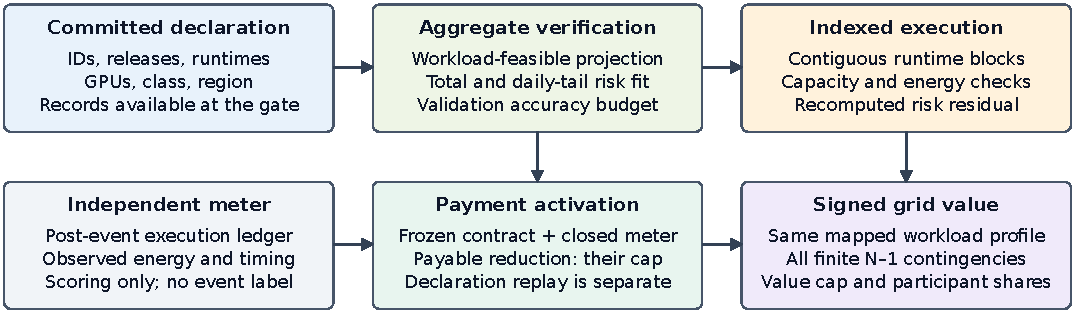
\includegraphics[width=\textwidth]{figures/fig0_framework.pdf}
\caption{Verification-to-settlement framework. Validation labels select the
counterfactual risk contract; locked execution truth is used only for scoring.
The right branch computes aggregate N--1 value and exact participant shares.}
\label{fig:framework}
\end{figure*}

\subsection{Sparse cumulative workload-state verifier}

For statistical estimate $\widetilde p$ and each predeclared penalty $\rho_\ell$,
the first-stage program solves
\begin{equation}
 \min_{x,y,z}\ \mathcal C_{\rm w}(x)+\rho_\ell\sum_{d,t}z_{dt}
 \quad {\rm s.t.}\quad
 z_{dt}\geq\pm(p_{dt}(x)-\widetilde p_{dt}),
 \label{eq:projection}
\end{equation}
subject to (\ref{eq:cumulative})--(\ref{eq:power}), with workload cost
$\mathcal C_{\rm w}$. The epigraph (\ref{eq:projection}) \cite{boyd2004convex} changes the objective,
not feasibility.
Six globally solved metadata schedules $p^{(\ell)}$ share identical arrivals
and constraints. A seventh causal Pareto projection is selected on validation
from the high-5-of-10 declaration target by a lexicographic rule over nRMSE,
false credit, under-credit, and $1-F_1$. A complete-ledger feasible-quantile projection is retained as
an external post-commitment comparator and is used only in the separate
payment hull. For a hull profile,
$\bar p=\sum_{\ell=1}^{L}\alpha_\ell p^{(\ell)}$, $\alpha\geq0$,
$\mathbf1^\top\alpha=1$, remains feasible because the common scheduling set is
convex.

The convex fit minimizes validation error plus total and daily-tail false-credit
exposure, measured by an empirical top-$m$ tail mean (the CVaR epigraph at effective level
$1-m/H$) \cite{rockafellar2000cvar}. Let $\ell^\star$ minimize contiguous-fold nRMSE and
let $B_h$ be the absolute daily false-credit exposure of the validation-selected
causal Pareto anchor on validation day $h$. This anchor differs from the external single-projection comparator.
For a candidate simplex profile define
$F_h(\alpha)=\sum_{n\in h}f_n$, where $f_n$ is the positive-part false
credit at sample $n$. Exposure is in MW-slots, without division by true credit. With
$m=\lceil(1-\gamma)H\rceil$ and reserve $\beta\in(0,1]$, solve
\begin{equation}
\begin{aligned}
\min_{\alpha,f,\nu,u}\quad
&\frac{\left\|\bar p-p^{0,\mathrm{decl}}\right\|_2^2}{N s_p^2}
 +\lambda\|\alpha\|_2^2
 +\omega_T\frac{\sum_{h=1}^{H}F_h}{S_T}\\[-2pt]
&\hspace{1.5em}+\omega_C\frac{\nu+m^{-1}\sum_{h=1}^{H}u_h}{S_C},
\end{aligned}
\label{eq:riskobjective}
\end{equation}
In (\ref{eq:riskobjective}),
$s_p^2=\max\{N^{-1}\|p^{0,\mathrm{decl}}\|_2^2,\epsilon\}$,
$S_T=\max\{\sum_hB_h,\epsilon\}$, and
$S_C=\max\{m^{-1}\sum_{h\in\operatorname{tail}_\gamma}B_h,\epsilon\}$.
Single-axis ablations remove one term and its constraint; the locked joint fit
uses $\omega_T=1.00$, $\omega_C=0.50$, $\gamma=0.75$, and $\lambda=10^{-8}$.
Both preferences and the total/tail budgets (\ref{eq:totalrisk})--(\ref{eq:cvar})
are frozen before locked scoring:
\begin{align}
 \sum_{h=1}^{H}F_h(\alpha)&\leq\beta\sum_{h=1}^{H}B_h,\label{eq:totalrisk}\\
 {\rm Tail}_{m}\!\left(F_h(\alpha)\right)
 &\leq\beta{\rm Tail}_{m}(B_h).\label{eq:cvar}
\end{align}
The positive part is represented without differentiating through a sort. For
each event sample $n$ and validation day $h$, introduce
$f_n\geq0$, a CVaR threshold $\nu\geq0$, and tail slacks $u_h\geq0$:
\begin{align}
 f_n&\geq p^\alpha_n-p^{(\mathrm{sim})}_n-r^{(\mathrm{sim})}_n,\\
F_h(\alpha)&=\sum_{n\in h}f_n,\\
 F_h(\alpha)-\nu-u_h&\leq0,\\
 \nu+\frac{1}{m}\sum_h u_h
 &\leq\beta\,\mathrm{Tail}_{m}(B_h).
 \label{eq:riskepigraph}
\end{align}
Equation~(\ref{eq:riskepigraph}) uses the same top-$m$ convention as scoring.
Here $r^{(\mathrm{sim})}_n=[p^0_n-p^{(\mathrm{sim})}_n]_+$, so its false-credit
row equals the nested-positive-part definition. To preserve the point-estimate metric, let
$q_\ell=N^{-1/2}\|p^{(\ell)}-p^{0,\mathrm{decl}}\|_2$ and
$q_\star$ denote the RMS error of the validation-selected causal Pareto
reference. The simplex additionally satisfies the linear sufficient condition
\begin{equation}
 \sum_{\ell=1}^{L}\alpha_\ell q_\ell
 \leq \sqrt{1+\varepsilon_{\rm acc}}\,q_\star,\qquad
 \varepsilon_{\rm acc}=0.10 .
 \label{eq:accuracycertificate}
\end{equation}
The triangle inequality proves (\ref{eq:accuracycertificate}) sufficient for
10\% validation-MSE non-inferiority. The sparse QP is solved with SciPy
trust-constr; Karush--Kuhn--Tucker stationarity and all primal residuals are
recomputed. Four contiguous folds select $\beta$ only when every training
contract is feasible. A separate payment projection targets $\bar p$ under
\begin{equation}
p^{\rm safe}_{dt}\leq p^{(\ell^\star)}_{dt}. \label{eq:envelope}
\end{equation}
This event-slot cap (\ref{eq:envelope}) never replaces the risk-fitting profile.

\paragraph{Binding-tail revision test.}
To distinguish a hard risk constraint from a soft objective preference,
Experiment~31 keeps the candidate hull and 10\% accuracy neighborhood but
replaces (\ref{eq:accuracycertificate}) with the exact convex row
$N^{-1}\|\bar p-p^0\|_2^2\leq(1+\varepsilon_{\rm acc})q_\star^2$. Starting from the exact-MSE total-only optimum, the
validation total budget is 1.10 times its exposure. A second solve minimizes
the top-$m$ tail under that budget. The primary tail cap is the midpoint
between this minimum and the total-only tail; quarter- and three-quarter
points provide the frozen frontier. Its objective retains only MSE and total
exposure, so an active tail constraint has an identifiable role. A separate
control removes the old hard risk rows while preserving the old objective.
These are retrospective revision experiments motivated by previously inspected
locked results, not a new untouched holdout.

\paragraph{Two-sided credit band.}
To exclude a zero-credit envelope, tie a lower band to the fitted target. Define
$p^{\rm floor}_{dt}=\min\{p^{(\ell^\star)}_{dt},\bar p_{dt}\}$, where $\bar p$ is
the pre-projection validation fit. The event-slot constraints are
\begin{equation}
 p^{\rm floor}_{dt}-\varepsilon
 \leq p^{\rm safe}_{dt}\leq p^{(\ell^\star)}_{dt},
 \qquad (d,t)\in\mathcal D\times\mathcal E,
 \label{eq:twosided}
\end{equation}
In (\ref{eq:twosided}) we set $\varepsilon=0$; the upper profile proves
nonemptiness. The lower
side regularizes under-credit without an unseen-trace guarantee. The separate
meter cap (\ref{eq:meter_cap}) controls realized payable credit.

\paragraph{Decision-time information boundary.}
A gate removes all post-gate arrivals before refitting the matched-information
target. The locked protocol uses slot 62, 30 minutes before the first event
slot, and a no-tariff LP freezes the contract baseline with a predeclared 3-MWh
minimum of participating event-window service. A second LP applies the selected
positive DR price to the same masked ledger while carrying unexpired state.
Reserved future jobs cannot be credited, and the tariff plan is scored against
the closed meter through (\ref{eq:meter_cap}). The independent execution trace
is read only in the scoring pass.

An earlier-days-only quantile reserve is evaluated separately for planning;
unsubmitted future jobs are never payment eligible. Sparse cumulative states
have $O(|\mathcal S||\mathcal K||\mathcal D||\mathcal T|)$ nonzeros.
Two lexicographic LPs minimize L1 error and then operating cost using HiGHS
\cite{huangfu2018highs}. Figure~\ref{fig:methoddetail} summarizes the stages.

\begin{figure}[t]
\centering
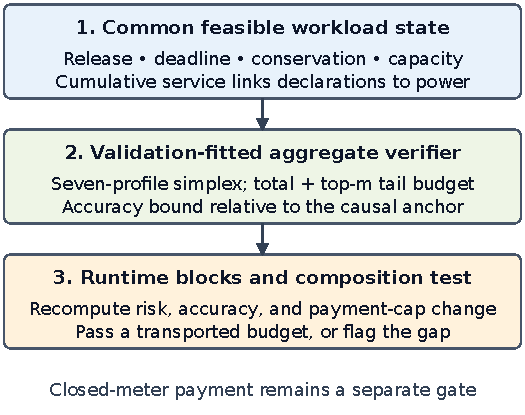
\includegraphics[width=\columnwidth]{figures/fig_method_detail.pdf}
\caption{Verification and execution stages. Aggregate feasibility, validation
risk, and runtime feasibility are distinct certificates. The composition test
recomputes their compatibility before network valuation or payment.}
\label{fig:methoddetail}
\end{figure}

\subsection{Runtime-complete execution and composition}

Let job $j$ have release $r_j$, requested GPUs $g_j^{\rm req}$,
declared runtime $R_j$ slots, fixed region $s_j$, and service endpoint
$d_j=r_j+R_j+B$, where $B$ is a precommitted queue allowance. With GPU
nameplate $\bar p_{\rm GPU}$, Define the runtime-complete entitlement
\(E_j^{\rm run}=R_jg_j^{\rm req}\bar p_{\rm GPU}\dt\). The indexed service
variable \(u_{j\tau}\) is the energy assigned to job \(j\) in interval \(\tau\),
and the executable witness requires one contiguous fixed-rate block of exactly
\(R_j\) slots. Let \(w_{\rm batch}\) be the predeclared waiting-cost coefficient per
MWh-slot, and \(r^{\rm DR}\) the event service tariff. Define
\(c_j=g_j^{\rm req}\bar p_{\rm GPU}\dt\) and
\(\Theta_j=\{r_j,\ldots,d_j-R_j\}\). For each admissible start \(\theta\),
a binary \(z_{j\theta}\) selects the block and
\(u^{j\theta}_{\tau}=c_j\mathbf1\{\theta\leq\tau<\theta+R_j\}\). The exact
start-time mixed-integer linear program (MILP) is
\begin{equation}
\begin{aligned}
 &\sum_{\theta\in\Theta_j}z_{j\theta}=1,\qquad z_{j\theta}\in\{0,1\},\\
 &u_{j\tau}=\sum_{\theta\in\Theta_j}u^{j\theta}_{\tau}z_{j\theta},\qquad
   \sum_{j:s_j=d}u_{j\tau}\leq\bar P_d\dt,\\
 &\min_z\ \sum_{j,\theta\in\Theta_j}z_{j\theta}
   \sum_{\tau}\left[w_{\rm batch}(\tau-r_j)+r^{\rm DR}\mathbf1\{\tau\in\mathcal E\}\right]u^{j\theta}_{\tau}.
\end{aligned}
\label{eq:jobindexed}
\end{equation}
Every selected block in (\ref{eq:jobindexed}) enforces runtime completion, contiguity, and the GPU
nameplate. Independent per-job enumeration solves the displayed MILP exactly
only if the combined minimizers satisfy every regional capacity row. Binding
capacity requires the coupled MILP; separability is not presumed. Waiting cost is charged at every service interval, not only the start. The training-calibrated entitlement $\widehat E_j$ is carried on the same
blocks only as a diagnostic; it is not measured consumption and does not
replace the runtime/nameplate commitment.
The risk target is linked through a fixed
regional slot price. Because the statistical and nameplate ledgers have
different scales, define the locked window set
$\mathcal W_{\rm lock}=\bigcup_{h\in\mathcal H_{\rm lock}}
\{96h,\ldots,96h+95\}$. The declaration energy active in this set is
\begin{equation}
 E_{\rm act}(\mathcal W_{\rm lock})=
 \sum_{j\in\mathcal J_{\rm sub}}E_j^{\rm dec}
 \frac{|[r_j,r_j+R_j)\cap\mathcal W_{\rm lock}|}{R_j},
 \label{eq:activewindow}
\end{equation}
In (\ref{eq:activewindow}), $E_j^{\rm dec}$ is either the nameplate upper entitlement or the
calibrated central entitlement. This overlap integral includes carry-in jobs
and uses only submit-time fields. Let
$\widetilde p^{\rm risk}_{dht}=P_d^{\rm fix}+\gamma_+[\bar p^{\rm risk}_{dht}-P_d^{\rm fix}]_+$,
with $\gamma_+=E_{\rm act}(\mathcal W_{\rm lock})/\sum_{d,h,t}
[\bar p^{\rm risk}_{dht}-P_d^{\rm fix}]_+\dt$. For locked day $h$, region
$d$, and interval $t$, define the fixed normalized slot-price heuristic
$\pi_{dht}=r^{\rm DR}[\widetilde p^{\rm risk}_{dht}-P_d^{\rm fix}]_+ /
\widetilde\Pi_{\max}$, where $\widetilde\Pi_{\max}=\max_{d,h,t}
[\widetilde p^{\rm risk}_{dht}-P_d^{\rm fix}]_+$. Re-enumerating every
declaration-feasible block with the waiting, event-tariff, and $\pi_{dht}$
terms produces the exact minimizer of this finite linear-price objective. The
optimality statement concerns the declaration-feasible policy; equality to the
aggregate target is a separate primal residual. The bridge therefore records,
for every locked day,
\begin{equation}
 \begin{aligned}
 e^{\rm br}_{dht}&=p^{\rm exec}_{dht}-\widetilde p^{\rm risk}_{dht},\\
 \mathrm{nRMSE}_{\rm flex}&=
 \frac{\|e^{\rm br}\|_2}{\max\{\|\widetilde p^{\rm risk}-P^{\rm fix}\|_2,\epsilon\}}.
 \end{aligned}
 \label{eq:bridge_residual}
\end{equation}
Equation~(\ref{eq:bridge_residual}) defines the executable-profile residual and
its flexible relative-L2 measure, alongside the total-load normalization.
The positive normalization cancels from the slot price, so active-window
scaling changes target magnitude but not the selected starts. A high target
load receives a high positive cost; this is the objective of the archived slot-price comparator; it is not a
derived target-tracking dual price. The resulting risk and accuracy must be
recertified after execution.
For the job-to-network certificate, the indexed witness is mapped without a
second optimization. To avoid overloading the deadline endpoint $d_j$, let
$\mathcal J_{sk\delta}$ be the ledger partition whose source, class, and
declared destination labels are $s,k,\delta$; Experiment~27 uses the native
assignment $\delta=s_j$ and therefore has no outcome-dependent migration:
\begin{align}
 x^{\rm job}_{sk\delta\tau}&=\sum_{j\in\mathcal J_{sk\delta}:\,r_j\leq\tau<d_j}
 u_{j\tau},\\
 p^{\rm job}_{\delta\tau}&=P_\delta^{\rm fix}+\dt^{-1}X^{\rm job}_{\delta\tau},\qquad
 X^{\rm job}_{\delta\tau}=\sum_{s,k}x^{\rm job}_{sk\delta\tau}.
 \label{eq:jobnetworkcoupling}
\end{align}
Equation~(\ref{eq:jobnetworkcoupling}) is reconstructed from the indexed
blocks before valuation; no independently refitted aggregate receives the
job witness's certificate. Aggregate migration remains a separate control.
Deferral and migration costs follow
\cite{cao2022flexibility,cao2024nonwire}, \cite{zhang2023receding}.

\paragraph{Residual-to-risk composition.}
Fix a baseline $b$, executable profile $x$, model reference $r$, and meter
$m$ on the same samples and scale. The nested positive parts in
(\ref{eq:falsecredit}) simplify to
$F_h(b)=\dt\sum_{n\in h}[b_n-\max\{m_n,r_n\}]_+$.
Let $\delta_h=\dt\sum_{n\in h}|x_n-b_n|$ and let
$T_m$ average the largest $m$ daily values. Then
\begin{align}
 F_h(x)&\leq F_h(b)+\delta_h,\label{eq:compose_daily}\\
 \sum_hF_h(x)&\leq\sum_hF_h(b)+\sum_h\delta_h,\nonumber\\
 T_m(F(x))&\leq T_m(F(b))+T_m(\delta),\label{eq:compose_tail}\\
 \mathrm{RMSE}(x,r)&\leq\mathrm{RMSE}(b,r)+\mathrm{RMSE}(x-b).
 \label{eq:compose_accuracy}
\end{align}
The positive part is 1-Lipschitz, proving (\ref{eq:compose_daily}). Summation gives
the total bound; monotonicity and subadditivity of the top-$m$ mean give
(\ref{eq:compose_tail}); (\ref{eq:compose_accuracy}) is the triangle inequality. Thus
residual budgets can certify transport, while an exact recomputation can pass
when the sufficient bound is conservative. Identity and energy conservation
alone cannot imply these inequalities meet a specified risk budget.

For payable credit $q=\min\{[x-m]_+,[b-m]_+\}$, its false credit is bounded
pointwise by that of $b$. Therefore the intersection preserves total and tail
risk whenever $b$ passes on the same reference, meter, and sample set. It does
not preserve executable-profile accuracy or identify a physical no-event
counterfactual. Experiment~31 checks both the uncapped execution certificate
and the separate capped-credit certificate without conflating their outcomes.


\paragraph{Direct risk-constrained runtime optimization.}
The composition inequalities permit failure; a stronger alternative puts the
risk rows inside the full-runtime MILP. Experiment~32 fixes declaration-only
reference and response scenarios, adds total and top-$m$ risk rows, and tests
an exact MSE budget on the same jobs. For a common GPU power quantum $q$, normalized integer load $z$ and
normalized target $\zeta$ admit the exact squared-error epigraph
\begin{equation}
 v\geq(2k-2\zeta)z+\zeta^2-k^2,\quad k=0,\ldots,\bar z.
 \label{eq:lattice_mse}
\end{equation}
For any feasible integer $z$, the row $k=z$ attains $(z-\zeta)^2$, while every
other row is below it. Thus (\ref{eq:lattice_mse}) with an MSE budget or
minimum-MSE objective enforces the exact error; the physical MSE is
$q^2\sum v/N$ over $N$ event samples.
The diagnostic retains infeasible contracts and minimizes achievable MSE
under unchanged risk/capacity rows. It is a finite known-scenario certificate,
not foresight of an unknown future meter.

\subsection{Signed nodal and N--1 settlement}

Let $\lambda^0\in\partial V(p^0)$ be the nodal demand-value subgradient.
Signed linear settlement is $({\lambda^0})^\top(p^0-p^1)$, while
(\ref{eq:value}) is the realized signed system-value benchmark. Convexity
\cite{boyd2004convex} gives

\begin{equation}
 0\leq(\lambda^0)^\top(p^0-p^1)-\Delta V
 =V(p^1)-V(p^0)-(\lambda^0)^\top(p^1-p^0).
 \label{eq:bregman}
\end{equation}
Thus the linear rule upper-bounds exact value in the polyhedral market model;
equality requires a common supporting subgradient.

For market-compatible remuneration, let $\mathcal W$ contain the complete response cycle from anticipatory shift
through recovery. Its space--time remuneration is

\begin{equation}
 \Pi^{\rm ST}=\dt\sum_{t\in\mathcal W}\sum_d
 \lambda^0_{dt}(p^0_{dt}-p^1_{dt}).
 \label{eq:spacetime}
\end{equation}
This is the nodal virtual-link structure of
\cite{zhang2020virtuallinks,zhang2022remunerating}; summing site payments
reproduces (\ref{eq:spacetime}).

Space--time energy remuneration is one component of the contracted DR
product. Let $\mathcal D^{\rm part}$ be the predeclared participating sites,
$\mathcal E$ the event intervals, and $r^{\rm DR}$ the cleared service price.
The signed delivered capacity service and total operator value are
\begin{align}
 Q^{\rm cap}&=\dt\sum_{d\in\mathcal D^{\rm part}}\sum_{t\in\mathcal E}
 (p^\emptyset_{dt}-p^1_{dt}), \label{eq:capacityservice}\\
 G&=r^{\rm DR}Q^{\rm cap}+\Pi^{\rm ST}, \label{eq:operatorvalue}
\end{align}
where $p^\emptyset$ is the minimum-cost no-event schedule on the same window.
Equation~(\ref{eq:capacityservice}) defines the bilateral capacity product and
need not equal trace-anchored
$p^0$; $\Pi^{\rm ST}$ debits spatial transfer and recovery. This signed service
model follows demand-response mechanism design \cite{satchidanandan2023twostage,chen2021incentive}.

For operator value (\ref{eq:operatorvalue}), define opportunity cost $C_{\rm opp}=\mathcal C_{\rm w}(x^1)-
\mathcal C_{\rm w}(x^\emptyset)$ and surplus $S=G-C_{\rm opp}$. A symmetric
Nash contract \cite{nash1950bargaining} activates iff $S\geq0$, transfers
$C_{\rm opp}+S/2$, and gives each party utility $S/2$. Nonactivation is the
zero-utility outside option. This bilateral transfer is separate from nodal
remuneration and exact dispatch value.
For the full-day ledger, the interval system amount is
$s_t=r^{\rm DR}\dt\mathbf1\{t\in\mathcal E\}\sum_dq^{\rm pay}_{dt}
+\Delta V_t$, where $q^{\rm pay}$ is in MW, $\dt$ is in hours, and
$\Delta V_t=\dt[V(p_t^0)-V(p_t^1)]$ is in USD. The economic ledger
$S^{\rm signed}=\sum_{t\in\mathcal W}s_t$ retains debits; the separate cash
presentation is $S^{\rm cash}=\sum_{t\in\mathcal W}[s_t]_+$. The floor is
applied to each system interval, not to independently allocated regional
values. Complete-cycle conservation gives
$\sum_{d,t\in\mathcal W}(p^0_{dt}-p^1_{dt})\dt=0$ within solver tolerance.

Before payment comparison, the submitted, frozen-contract, and closed-meter
reductions are intersected as follows:
\begin{equation}
q^{\rm pay}_{dt}=\min\{q^{\rm obs}_{dt},q^{\rm cap}_{dt}\},\qquad
 G=r^{\rm DR}\dt\!\sum_{d,t\in\mathcal E}q^{\rm pay}_{dt}+\Pi^{\rm ST}.
\label{eq:settlementchain}
\end{equation}
Equation~(\ref{eq:settlementchain}) is evaluated after meter closure.
Experiment~12 audits its budget balance; Experiment~27 instead stores
$q^{\rm replay}_{dt}=\min\{q^{\rm dec}_{dt},q^{\rm cap}_{dt}\}$ to certify
feasible network value. Experiment~30 records this role as declaration-only, and the
replay's signed/cash totals remain outside payable settlement until
$q^{\rm obs}$ is available.

Security-aware settlement augments (\ref{eq:sced}) with every finite
non-islanding single-line outage. If $L_{\ell k}$ is the LODF from outage $k$
to monitored line $\ell$, then
\begin{equation}
 -\bar f_\ell\leq
 (H_\ell+L_{\ell k}H_k)(C_gg-p)\leq\bar f_\ell,
 \quad \ell\neq k.
 \label{eq:n1}
\end{equation}
Equation (\ref{eq:n1}) is the standard preventive N--1 LODF formulation
\cite{tejada2018lodf}; every credible row uses native ratings. Islanding rows are
excluded because a connected single-reference PTDF cannot represent separate
islands, consistent with the DC/N--1 planning scope \cite{nerc2020tpl}.

\subsection{Finite-scenario N--1 value-component certificate}

The pointwise envelope controls energy but not network payment because spatial
loads can activate different security constraints. Let $\mathcal P=\operatorname{conv}
\{p^{(1)},\ldots,p^{(L)}\}$ be the feasible-profile hull and
$p^{\rm cap}\in\mathcal P$ the validation-selected projection. Its penalty is
separate from the payment-target penalty; the feasible-quantile projection is an
external comparator. Let $\Xi_5$ be the 1st, 10th, 50th, 90th, and 99th
calibration-validation GPU-energy ratios from independent telemetry
\cite{samsi2021supercloud}. For facility profile $p^{\rm fac}_{dt}$, fixed demand
$P^{\rm fix}_d$, scale $s_{\rm dc}$, and factor $\xi$,

\begin{equation}
 p^{\rm dc,\xi}_{dt}=s_{\rm dc}\bigl(P^{\rm fix}_d+\xi[p^{\rm fac}_{dt}-P^{\rm fix}_d]\bigr),
 \qquad p^{\rm fac}_{dt}\geq P^{\rm fix}_d .
 \label{eq:fixedflexconversion}
\end{equation}
The scale uses the calibration-validation $q_{99}$ flexible peak, keeping the
fixed component invariant to $\xi$; raw endpoints remain activation scenarios.
The injection is $M p^{\rm dc,\xi}_t$, with superscripts $\alpha$ and ``cap''
applying (\ref{eq:fixedflexconversion}) to $p^\alpha$ and $p^{\rm cap}$. For
each settlement day, the \PaymentSafe{} defines
$B_\xi^{\rm cap}=\dt\sum_{t\in\mathcal E}
V_{N-1}(p_t^{\rm native}+M p_t^{\rm dc,\xi,cap})$ and solves
\begin{align}
\operatorname{lexmin}_{\alpha,e,\eta,\{g_t^\xi\}}\quad&
 \left(\sum_{d,t\in\mathcal E}e_{dt},-\eta\right)
 \label{eq:paymentcert}\\
\mathrm{s.t.}\quad&
 p^\alpha=\sum_{\ell=1}^{L}\alpha_\ell p^{(\ell)},\nonumber\\
&\alpha\geq0,\quad\mathbf1^\top\alpha=1,\quad 0\leq\eta\leq1,\nonumber\\
&e_{dt}\geq\pm(p^\alpha_{dt}-p^{\rm safe}_{dt}),\nonumber\\
&g_t^\xi\ \text{satisfies (\ref{eq:sced}) and (\ref{eq:n1})},\nonumber\\[-2pt]
&\hspace{2em}\text{with }p_t=p_t^{\rm native}+M p_t^{\rm dc,\xi,\alpha},\nonumber\\[-2pt]
&\hspace{7.5em}t\in\mathcal E,\quad \xi\in\Xi_5,\nonumber\\
&\dt\sum_{t\in\mathcal E}\sum_iC_i(g_{it}^\xi)\nonumber\\[-2pt]
&\hspace{2em}\leq(1-\eta)B_\xi^{\rm cap},
\quad \xi\in\Xi_5.\nonumber
\end{align}
The epigraph in (\ref{eq:paymentcert}) is solved by two global LPs: trajectory error is
minimized first, then the common fractional margin $\eta$. Feasibility is the
N--1 upper bound and $p^{\rm cap}$ proves nonemptiness. Hence, for any
$\xi\in\Xi_5$ and realized load $p^{1,\xi}$, the daily dispatch-value
component obeys
\begin{multline}
\sum_{t\in\mathcal E}\dt
[V_{N-1}(p_t^{\rm native}+M p_t^{\rm dc,\xi,\alpha})
-V_{N-1}(p^{1,\xi}_t)]\\
\leq\sum_{t\in\mathcal E}\dt
[V_{N-1}(p_t^{\rm native}+M p_t^{\rm dc,\xi,cap})
-V_{N-1}(p^{1,\xi}_t)].
\label{eq:paymentdominance}
\end{multline}
The realized cost cancels, so this is a samplewise value-component certificate
without execution truth. Inequality~(\ref{eq:paymentdominance}) does not bound the capacity term, linear
space--time transfer, or positive cash floor of the entire contract. The hull contains six first-stage projections and feasible quantile. The
network contract targets the joint-risk profile but is excluded from its fit.

A separate continuous-segment audit minimizes dispatch value over the segment
between the frozen cap and certified profile. A joint LP gives its minimum;
convexity places the maximum at an endpoint when the realized counterfactual
is fixed. This does not establish a continuous-conversion guarantee when the
realized load also changes. The repository supplement gives the interval
formulation and its independent-resolution checks.

\subsection{Participant allocation}

For participants $N$, let $v(S)$ be signed dispatch value when coalition $S$
moves from baseline to actual demand. The exact allocation is
\begin{equation}
 \phi_i(v)=\sum_{S\subseteq N\setminus\{i\}}
 \frac{|S|!(|N|-|S|-1)!}{|N|!}
 [v(S\cup\{i\})-v(S)].
 \label{eq:shapley}
\end{equation}
The signed allocation (\ref{eq:shapley}) \cite{shapley1953value} is efficient:
$\sum_i\phi_i=v(N)$ if $v(\varnothing)=0$. All coalitions are evaluated for
four sites and eight portfolios; exchangeable site slices reduce larger
contracts to count states. This allocation does not change physical
feasibility or the meter gate.

\subsection{Scope of the composed certificate}

The common ledger preserves provenance, not automatically every guarantee.
For incidence $B_{dj}=\mathbf1\{s_j=d\}$ and bus map $M$, the implementation
checks job energy $\sum_\tau u_{j\tau}=E_j^{\rm run}$, regional equality
$X_{d\tau}=\sum_jB_{dj}u_{j\tau}$, and nodal mapping
$p_{b\tau}=P^{\rm fix}_{b\tau}+\dt^{-1}\sum_dM_{bd}X_{d\tau}$.
These equalities ensure that the valued profile is the indexed executable
profile. If dispatch value is $L_V$-Lipschitz on the committed feasible
polytope, a mapping residual $r^{\rm map}$ incurs at most
$L_V\|r^{\rm map}\|_1$ value error.

The workload projection and its convex hull inherit only the aggregate
feasible set. The accuracy bound holds on validation, and the value cap holds
only on its frozen conversion scenarios. Runtime completion, information
availability, transported risk, network feasibility, and meter activation are
therefore checked as distinct predicates on one profile. Passing a digest or
an optimizer residual alone is insufficient for end-to-end activation.

\section{Experimental Design}\label{sec:design}

\subsection{Data and predeclared information sets}

BurstGPT supplies 5,188,507 successful requests
\cite{wang2024burstgpt}; MIT Supercloud supplies 75,326 valid scheduler
submissions and 71,128 positive-energy executions
\cite{samsi2021supercloud}. The aggregate tensor contains 68,662 executions
with valid intervals. Chronological fitting uses the first 40 complete days;
validation uses days 45--60 and locked scoring uses days 61--114. Submit-time
features define decisions. Measured intervals and DCGM energy are opened only
for scoring, with no utility-event label.

Aggregate deferral windows are 0, 4, and 512 slots. Each scenario region has a
6-MW fixed component and 118-MW flexible capacity. For the runtime witness,
$\bar p_{\rm GPU}=0.001$ MW/GPU, $B=96$ slots, and an unlimited Slurm
runtime maps to 128 slots; finite declarations are retained. Runtime and queue
allowance are separate: Slurm timelimit is not a submit-to-completion deadline.
The runtime/nameplate entitlement, training-calibrated central energy, measured
GPU energy, and network-scaled facility demand remain separate quantities.
Population and calibration joins are documented in the supplement.

Geography is unobserved. Four regions are assigned by a predeclared
feature-stratified round robin; the spatial panel exhausts 24 permutations,
two concentration controls, and three penetrations at a 0.75 native-load
multiplier. Payment-network scaling uses the calibration-validation flexible
$q_{99}$ peak at a declared 4\% penetration, with the fixed component held
separate. Five measured conversion ratios span 0.583--5.321; neither
normalization nor nameplate coverage establishes a measured 100-MW facility.
Topologies, ratings, and costs follow the Power Grid Library (PGLib), MATPOWER, and RTS-24
\cite{babaeinejadsarookolaee2021pglib,zimmerman2011matpower}, \cite{grigg1999rts}.

\subsection{Comparators and experimental questions}

The aggregate panel compares history-only estimators, declaration-feature
estimators, synthetic control, a single feasible projection, and a
validation-selected causal Pareto anchor. The proposed \RiskSafe{} combines
total and daily-tail preferences; ``total-only'' and ``tail-only'' are
independently solved ablations. The \PaymentSafe{} is a separate network-value
cap, never an additional risk-fitting candidate. Complete-ledger quantile
comparators are explicitly ex-post. Structural scheduling translations use
matched constraints but are not reproductions of published software
\cite{cao2022flexibility,chen2021idccoupling}.

Four contiguous leave-block-out validation folds select projection penalties
and risk reserve; these are not rolling-origin folds. The joint QP fixes
$\omega_T=1$, $\omega_C=0.5$, $\gamma=0.75$, $\lambda=10^{-8}$, and the
10\% validation-MSE budget. Tail statistics always average exactly the worst
$m=\lceil(1-\gamma)H\rceil$ days, including in bootstrap samples with ties.
Thus the locked 54-day statistic uses 14 days and effective level
$1-14/54=0.741$, rather than exact empirical CVaR at 0.75.

Three-day moving-block percentile intervals are exploratory and unadjusted;
block-length sensitivity is reported. The separate exact block-sign tests
use all $2^{18}$ assignments and Holm-adjusted $p$-values
\cite{kunsch1989bootstrap,holm1979multiple}. Means improving together do not
imply simultaneous statistical significance. Model- and source-hash checks
bind results to the saved profiles; recomputation using a shared selector is
distinguished from an independent algorithmic cross-check.

The experiment index supports four questions: whether risk control improves
verification; whether the guarantee survives runtime execution under one
information set; whether signed network accounting adds value; and whether
security results retain a common denominator. The original witness and
bridge (Experiments~27--30), composition test (Experiment~31), and matched-gate
capacity test (Experiment~32) retain their distinct roles. The AC fixed-plan
panel freezes non-reference active generation after intact dispatch, allowing
reference balance, reactive output, and voltage recourse. Its six snapshots
are days 61, 88, and 114 at slots 64 and 71, not independent operating days.
All numerical backends are single-threaded; revision tests use at most two
concurrent CPU workers.

\section{Results}\label{sec:results}

\subsection{Verification accuracy and risk trade-offs}

The mechanism-isolation experiment confirms the economic motivation. At
\$150/MWh and call probability 0.35, strategic scheduling increases the
historical event baseline by 8.223 MWh, of which 44.458 of 55.452 credited MWh
are unsupported by the model-reference reduction. The marginal threshold
(\ref{eq:threshold}) agrees with independent strategic optimization in all 56
price/probability cells (Experiment~1).

Table~\ref{tab:base} separates the verification trade-off from deployment.
The \RiskSafe{} lowers mean false credit from 2.470 to 0.780 MWh/day relative
to the single projection, and improves its other three means. Its nRMSE
improvement is not significant in the reported Holm-adjusted test
($p=0.158$; three-day interval $[-0.006,0.080]$). Block-sum autocorrelation
is 0.727 for this contrast, so the supplied block-length sensitivity matters.
The causal Pareto anchor is more accurate and has less under-credit; the
total-only ablation has better means on all four metrics. The data therefore
do not establish that adding the old tail preference improves prediction.

\begin{table}[t]
\centering
\caption{Complete-ledger mechanism-isolation results, 54-day means.
Credit columns are MWh/day; nRMSE and $F_1$ are dimensionless.}
\label{tab:base}
\footnotesize
\setlength{\tabcolsep}{3pt}
\begin{tabular}{@{}lrrrr@{}}
\toprule
Method & nRMSE & \shortstack{False\\credit} & \shortstack{Under-\\credit} & $F_1$\\
\midrule
High-5-of-10 & 1.586 & 41.220 & 11.169 & 0.572\\
History ridge & 1.038 & 21.906 & 25.226 & 0.545\\
History boosting & 1.011 & 20.977 & 26.401 & 0.534\\
History extra trees & 1.090 & 26.629 & 18.176 & 0.597\\
Declaration boosting & 0.774 & 9.183 & 21.528 & 0.640\\
Ex-post decl. boosting & 0.750 & 9.171 & 20.817 & 0.643\\
Ex-post quantile & 1.337 & 0.591 & 54.391 & 0.237\\
Synthetic control & 0.782 & 9.394 & 21.678 & 0.676\\
Feasible quantile & 1.344 & 0.098 & 52.647 & 0.225\\
Single projection & 0.943 & 2.470 & 26.812 & 0.463\\
Causal Pareto anchor & 0.691 & 1.895 & 17.024 & 0.699\\
Total-only & 0.892 & 0.646 & 26.372 & 0.549\\
Tail-only & 0.905 & 0.817 & 26.541 & 0.533\\
Original joint & 0.902 & 0.780 & 26.506 & 0.536\\
\midrule
Exact-MSE total-only & 0.949 & 0.565 & 28.481 & 0.506\\
\textbf{Active tail} & 0.945 & 0.540 & 28.384 & 0.511\\
\bottomrule
\end{tabular}
\vspace{3pt}
\parbox{\columnwidth}{\footnotesize Complete-ledger rows are ex-post information
comparators. High-5-of-10 is not workload-feasible. The causal anchor and
single projection are distinct validation targets. The final two rows use the
exact-MSE neighborhood.}
\end{table}


The validation joint MSE is 200.575 MW$^2$, below its 207.825-MW$^2$ budget;
stationarity and primal residuals are $9.69\times10^{-10}$ and
$1.11\times10^{-16}$. Both old risk budgets have positive slack. Removing
only those rows with the objective unchanged leaves essentially the same
solution, confirming that their presence does not explain the old fit.

The binding-tail revision instead makes the tail row active (slack
$4.63\times10^{-8}$, dual 0.0537). Against its matched exact-MSE total-only
control, it reduces locked mean false credit from 0.565 to 0.540 MWh/day and
top-14-day tail from 1.944 to 1.861 MWh. Its nRMSE is 0.945 versus 0.949,
and $F_1$ is 0.511 versus 0.506. The paired tail difference has an
unadjusted 95\% block-bootstrap interval $[-0.182,0.006]$ MWh, including
zero. Compared with the original joint fit, this variant sacrifices accuracy
and recall for lower false credit. This is a measured frontier, not a
confirmatory superiority result (Experiment~31; Fig.~\ref{fig:result_certificates}, left).

Independent observed-meter replay is less favorable: event-window MAE is
6.880 MW for the joint-risk verifier, 7.038 MW for the single projection,
and 1.909 MW for feasible quantile (Experiment~20). Meter independence
prevents scoring leakage, but supplies no identified no-event counterfactual.

\begin{figure*}[t]
\centering
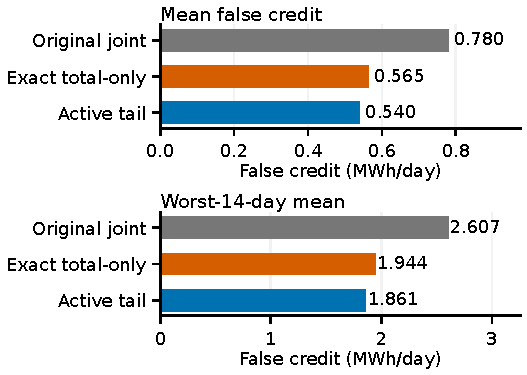
\includegraphics[width=0.49\textwidth]{figures/fig_risk_tail_tradeoff.pdf}\hfill
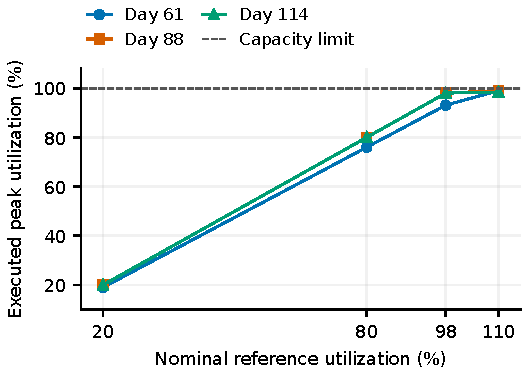
\includegraphics[width=0.49\textwidth]{figures/fig_runtime_capacity.pdf}
\caption{Risk control and coupled execution. Left: original joint and
exact-MSE controls on the retrospective 54-day panel; the active-tail versus
exact-total-only tail difference has an interval including zero. Right:
full-runtime, direct-risk schedules across the predeclared capacity scan.
Each plotted point is globally optimal for its finite model; no full-population
congestion claim is inferred from these 64-job cohorts.}
\label{fig:result_certificates}
\end{figure*}

\begin{table*}[t]
\centering
\caption{N--1 settlement error on a common physical response (USD/day).
Overpayment is the mean positive error; medians are absolute errors.}
\label{tab:settlement}
\footnotesize
\setlength{\tabcolsep}{5pt}
\begin{tabular}{llrrrrrr}
\toprule
& &\multicolumn{2}{c}{MAE}&\multicolumn{2}{c}{Median}&\multicolumn{2}{c}{Overpayment}\\
Panel & Settlement rule & Trace & Workload & Trace & Workload & Trace & Workload\\
\midrule
N--1 & Base-case exact &139.221&167.367&79.790&121.010&130.420&107.690\\
N--1 & N--1 linear &2.208&150.461&0.600&113.430&1.910&20.380\\
N--1 & N--1 exact &0.990&150.955&0.870&113.430&0.010&20.180\\
\bottomrule
\end{tabular}
\end{table*}

\subsection{Does the certificate survive execution?}

The full runtime witness covers 75,326 declarations and 7,306,622 admissible
starts. Saved-policy recomputation has zero start mismatches and an objective
residual of $2.27\times10^{-13}$ USD; it reuses the original selector and is
not an implementation-independent optimality test. Capacity utilization peaks
at only 0.444\%, so the scalable exact result concerns a nonbinding regime.
The original bridge's total-profile nRMSE is 0.030, but its flexible relative
L2 error is 1.581 and maximum discrepancy is 3.220 MW. The fixed 6-MW component masks this
mismatch in the total-load normalization.

The scale-aligned composition test makes the failed link explicit
(Experiment~31). Under the same archived nameplate affine scale, the target's
total false credit is 1.610 MWh and its tail is 0.100 MWh. Execution raises
these to 22.101 and 1.149 MWh, exceeding carried audit budgets of 4.168 and
0.235 MWh. Executed MSE is 0.857 MW$^2$ against a 0.304-MW$^2$ budget.
All three uncapped execution tests fail, despite exact job/network provenance.
The total budget scales the validation daily allowance to 54 days; it is an
audit threshold, not a generalization theorem.

Intersecting executable and target credit reduces total false credit to
0.804 MWh and tail to 0.055 MWh, passing both risk limits. It also removes
22.981 of 32.829 MWh of uncapped credit. This proves the intended distinction:
the payment-risk cap can work while the executable-profile certificate fails.
This panel uses a model-generated event meter and a locked-block scale;
it remains an ex-post mechanism audit, not deployable meter evidence.

The matched-gate panel uses slot 62, identical eligible arrivals and pre-gate
aggregate state, all four sites, a common modeled reference/response, and the
same 3-MWh service floor (Experiment~32). Its 13 methods retain all 70
validation/locked days. Joint, total-only, tail-only, and unconstrained fits
collapse to the selected causal projection: locked nRMSE 0.062, false credit
0.631 MWh/day, and recall/$F_1$ 0.790. The seven-candidate event hull has
rank two and only three distinct profiles, explaining the absence of an
incremental risk-module advantage. All methods' payable modeled credit is
3 MWh/day with zero modeled shortfall because of the binding floor and common
benchmark state; this is not measured delivery reliability.

The full-runtime capacity scan retains 64-job gate cohorts on days 61, 88,
and 114, with 32 pending and 32 already-running jobs each. Hypothetical
capacity changes; job power, runtime, deadlines, and all-slot constraints do
not. All 24 cost-only/direct-risk cells solve with zero gap, at achieved
peak utilizations of 19--99\% (Fig.~\ref{fig:result_certificates}, right). Risk rows change one high-load cell's false
credit from 0.00025 MWh to zero. The small cohort therefore demonstrates
coupled feasibility without repairing the 75,326-job bridge or establishing
full-scale congestion performance.

A sequential exact-match diagnostic imposes zero MSE and zero risk on six
high-utilization cells. Four pass; day-61 and day-114 contracts at nominal
utilization 1.10 are infeasible. Minimum-MSE solves under unchanged risk and
capacity certify achievable errors of $1.98\times10^{-7}$ and
$1.00\times10^{-6}$ MW$^2$ respectively, with zero gap in all six cells.
These retained failures show why runtime feasibility, risk, and accuracy
must be enforced together rather than inherited from an aggregate fit.


\subsection{Signed network value and security}

Signed netting changes settlement more than substituting exact value for its
linear approximation in the base case. For the trace-anchored rows in
Table~\ref{tab:settlement}, exact net-value MAE is \$151.719/day versus
\$360.580/day for nodal gross response. The paired netting improvement is
\$208.190/day (Holm-adjusted $p=3.89\times10^{-4}$); the linear-to-exact
change is \$0.671/day ($p=0.803$). All 5,616 interval/counterfactual instances
satisfy (\ref{eq:bregman}). These comparisons include the nodal-difference
space--time structure of virtual-link remuneration, while the exact benchmark
captures changes in dispatch regimes. For the workload response, base-case
MAE is \$455.865/day for exact signed value and \$421.677/day for nodal gross
response, so the trace-based gain is not universal.



The DC replay imposes all 37 finite non-islanding RTS-24 outages and reaches
maximum loading 1.000 p.u. Its denominator is not filtered using method
outcomes. The value-component cap passes all five frozen conversion scenarios
in 54 daily programs within $3\times10^{-11}$ USD. It does not dominate all
comparators: at the median/high conversion factors, the value-certified
verifier's MAEs are \$57.357/\$322.032 per day, versus the single projection's
\$41.141/\$231.841. On two held-out interior factors the joint-risk verifier
also has lower error than the value-certified profile. Contractual dominance
of a specified value cap and predictive accuracy are different properties.

The AC audit retains a common topology-connected domain of 10,332 cells:
37/38/35/177 outages for RTS-24/IEEE-30/IEEE-39/IEEE-118, three penetrations,
two methods, and six day--slot snapshots. It records 9,642 certified cells,
690 numerical unknowns, and no converged limit violations. The latter is
not a proof that unknown cells are feasible. The revision reuses 9,576
checksum-bound certificates and solves 756 cells, including matched controls.
On IEEE-30 outages 29 and 31, the proposed profile certifies all 36 cells;
the reference certifies 30, with six unknowns at 9\% penetration. Those six
outcomes no longer remove the reference's 30 successful cells. Native
screening is reported only as a subgroup; all methods retain the same primary
denominator. Six snapshots test the stated operating conditions, not an
annual reliability rate.

The original complete-cycle runtime replay reports signed value \$184.664 and
positive cash presentation \$283.470 across 5,184 cells. Keeping these ledgers
separate exposes negative network-value intervals that a cash floor would
hide. They are declaration-only values, not payments: the lineage audit
requires an independently closed meter before activation.

The old slot-62 gate and complete-ledger panels have different eligible
populations and scoring tasks. Their $F_1$ values of 0.080 and 0.536 cannot
be read as a matched causal degradation. The new matched protocol tests that
boundary directly. The existing 79-job binding-capacity experiment uses
calibrated service with a possible final partial slot; it does not establish
congestion performance for the full-runtime nameplate model. Neither public
trace replay nor synthetic geography can replace an identifiable utility
event, authenticated declarations, and a prospective deployment trial.

\section{Conclusion}\label{sec:conclusion}

This paper develops a contract-based connection between data-center workload
verification, runtime scheduling, and security-aware net-value settlement.
The exact convex fit makes tail-risk control identifiable, while residual
bounds and direct integer constraints establish when execution preserves a
specified contract. The coupled solver maintains job power, duration, and
deadlines and computes minimum achievable error when exact matching is
infeasible. Signed accounting and a common AC contingency denominator make
network-value and certification results comparable across methods. The
retrospective tests support a controllable risk--accuracy frontier and exact
finite-scenario feasibility checks. Prospective utility-event validation and
congested full-population testing remain the next steps for deployment.

\bibliographystyle{ieeetr}
\bibliography{references}

\end{document}
